\documentclass[12pt,letterpaper]{article}
\usepackage[utf8]{inputenc}
\usepackage{times}
\usepackage{authblk}
\usepackage{graphicx}

\title{StudyUp - Software Requirements and Planning}

\author[1]{Yukon Vinecki}
\author[2]{Chandler Petersen}
\author[3]{Calvin Todorovich}
\affil[1]{petercha, EECS - Oregon State University}
\affil[2]{vineckiy, EECS - Oregon State University}
\affil[3]{todorovc, EECS - Oregon State University}

% Don't indent new paragraphs, avoids unnecessary new lines
\usepackage[parfill]{parskip}
\begin{document}

\pagenumbering{roman}
\maketitle
\clearpage
\tableofcontents
\clearpage
\pagenumbering{arabic}

\section{Project Description}
We envision a web application, that will be easily accessible to college students. The StudyUp application aims to solve the problem of finding new people to study with in your classes. Since the alternative is making friends in person, students that are shy or introverted have a hard time finding help in classes, outside of TA's. There are other applications for creating groups, but they are aimed towards recreational activity. What sets StudyUp apart from any competition is the Canvas API. Using the Canvas API, we will be able to use students' data to show which classes they are in, which should streamline the process of finding a group as shown in figure \ref{systems}.

\begin{figure}[h]
  \centering
  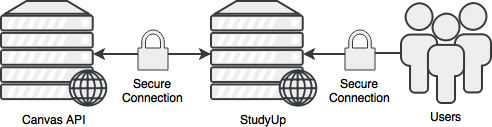
\includegraphics[width=20em]{Systems_Diagram.png}
  \caption{Systems Diagram}
  \label{systems}
\end{figure}

Since we envision StudyUp being a web application, we plan to use HTML5, CSS, and JavaScript, utilizing Bootstrap 4 for the front-end design and functionality of the web application. We chose these tools because they were the most comfortable to us and our background with CS 290.

Functional requirements, those related to the technical functionality of the system, include integration with individual students' Canvas accounts, the ability to start a study group, join a study group, the ability to login via Canvas, and potentially, the ability to search for existing study groups on canvas (this is more of a reach-goal). 

Some non-functional requirements, or requirements we are using to judge the operation of our application in certain conditions, are in the case that one student starts a study group, that another student will be able to join this group and find the location on the first student and be there at the correct time. Also, another requirement is, in the case a student wants to create a study group, they are able to create one under a subject corresponding to their class list in Canvas, as well as are able to set a time, date, location, length of meeting, and capacity for the group. 

StudyUp will incorporate a combination of a brief user manual as well as logically-placed help text throughout the interface. Each button will be labeled with its function, and the modal fields will each have an explanation for what kind of information they should contain and what will be done with it. When a user signs into the application, they will be greeted by a brief user manual that outlines the application's purpose and functionality, as well as how to use the system itself. This manual will also be available for reference via a button on the interface any time the user wishes to refer to it again. 

The major features of StudyUp that make it an effective and useful facilitator for study groups are: the ability for a student to create a study group at any location or time that other students can view and join, the interface with the student's Canvas account that allows them to easily create groups around their class subjects, the ability to join existing study groups, and the ability for the study group administrator to set specific information about a study group, including subject, time, location, length of meeting, group capacity, and study group objectives. Two features that we also hope to implement are the ability for students to search for active study groups on campus, a visual campus map of active study groups, and the ability to set recurring study group sessions. 

\section{Use Cases}

\subsection{User creates a Study Group}
\subsubsection{Goal}
The user ability to create a new study group for one of his classes.

This case is the most vital step in the entire application. Students need to create new groups in order to join them, so this is essential to the user and the very functionality of the application.

\subsubsection{Actors}
The user (a student) who wants to create a study group for a class.

\subsubsection{Pre/Post Conditons}
Preconditions for this case include the user must log in and Canvas support is implemented. Additionally, before a study group is created, the user must fill out the required information fields that define the subject of the study session, the time of meeting, the location, meeting length, the group objectives, and the capacity of the group.

Postconditions for this case are the user will have created a new study group, and they will be brought back to the main menu. At this point, the group will be "active," and any other users on the application will be able to view this study group and join it.

\subsubsection{Flow of Events}
From the main menu, they click a button to create a new study group. They choose a class for which this group will be associated with. The user sets a short title for the name of their group, like "ST 314 Midterm." We need to account for the user trying to input a string that is too long, or using special characters. The user then fills out the required fields for the study group, indicating time, date, location, objectives, length of meeting, and capacity. The user then confirms and activates the study group. 

\subsection{User joins a Study Group}
\subsubsection{Goal}
User will see a lists of classes they are taking and available study groups after they login and they will have the ability to select and join a group.

It is essential that the user is able to join a study group because  otherwise, study groups created by others would never get populated with other students, rendering this application useless. 

\subsubsection{Actors}
The user (a student) is looking for an existing study group for a specific class to join.

\subsubsection{Pre/Post Conditions}
Some preconditions for this case are the user must log in, and the Canvas API has been implemented. Also, there must be a study group currently active for the user to be able to join one. Additionally, the details of the group must correspond to the that of the user (i.e. they can make it to the group, its has not reached capacity, etc.)

Postconditions for this case include the user will be in a new study group, and they will be brought to a screen with all of the study groups that they currently occupy. The new study group should be at the top.The user can then go meet up with the group. 

\subsubsection{Flow of Events}
The user selects a "Join a study Group" button from the main menu. The user is presented with his current list of classes along with some of the study groups available. If there are more study groups than shown for a class the user can expand that given class to show all groups. The user then chooses a study group to join, and confirms.

\subsection{Viewing a Study Group}
\subsubsection{Goal}
The user ability to view information about a given study group, such as Objective, date/time, location, length of meeting, current group capacity, and maximum capacity.

\subsubsection{Actors}
In this use case, the user that is looking at potential study groups is the primary actor. 

\subsubsection{Pre/Post-Conditions}
Pre-conditions for this case is that there is at least one existing study group active, and that the study group administrator filled out the required fields to display information about the study group.

\subsubsection{Flow of Events}
The user will login to the application and look on page which will indicate what study groups are currently active. The user can then select one of these groups, which will bring up the details of this group via a new page or a modal. From there, the user can choose whether or not to join the group. 

\subsection{Most Important Scenarios}
These use cases cover the most important scenarios because they embody the primary functionality of the application. These use cases are going to be what the user is most likely, as well as most frequently, going to do. Therefore, they are the most important and should be given primary focus. If a user is using the application to begin with, this implies that they either want to create or join a study group. This covers the first two use cases. The third use case is important as well, as it outlines the scenario in which a user looks at what groups are available, but does or does not choose to join a group, a decision based upon the information given by viewing a group. 

\subsection{Main Error Scenarios and Remedies}
The main error scenarios include. The user attempting to create a study group for a class that does not exist in canvas (or just entering an invalid string for a search term). Users not ending their study group once the group is done studying (displaying an active group that no longer exists). Joining groups for classes for which they are not currently enrolled. Finally attempting to access the site while Canvas API is unavailable.

Remedies for the above errors in use respectively include. Checking to see if the group the user attempts to create is a valid class, and then displaying an error message if it is not (as well as checking to make sure entered strings are valid). Implementing a "timeout" feature, so the group will only be be displayed as active for as long as the "length" is specified. Making sure to check to see if the group the user attempts to join is valid considering the classing for which they are currently enrolled, and alerting the user in the case they try to join a non-valid group. If the Canvas API is unavailable, preventing authentication and other features, the site will display a message to the users notifying them that the website is currently unavailable.

\section{Planning}
\subsection{Milestones/Tasks}
This project has three milestones, UI Complete, Functionality Implemented, and Core Features Complete. These milestones focus on the stages of development where the dependencies to begin work on the next task are complete. A detailed breakdown of tasks and milestones can be found in the schedule.

\clearpage
\subsubsection{Schedule}
Figure \ref{gantt} below is the current Gantt schedule.

\begin{figure}[h]
  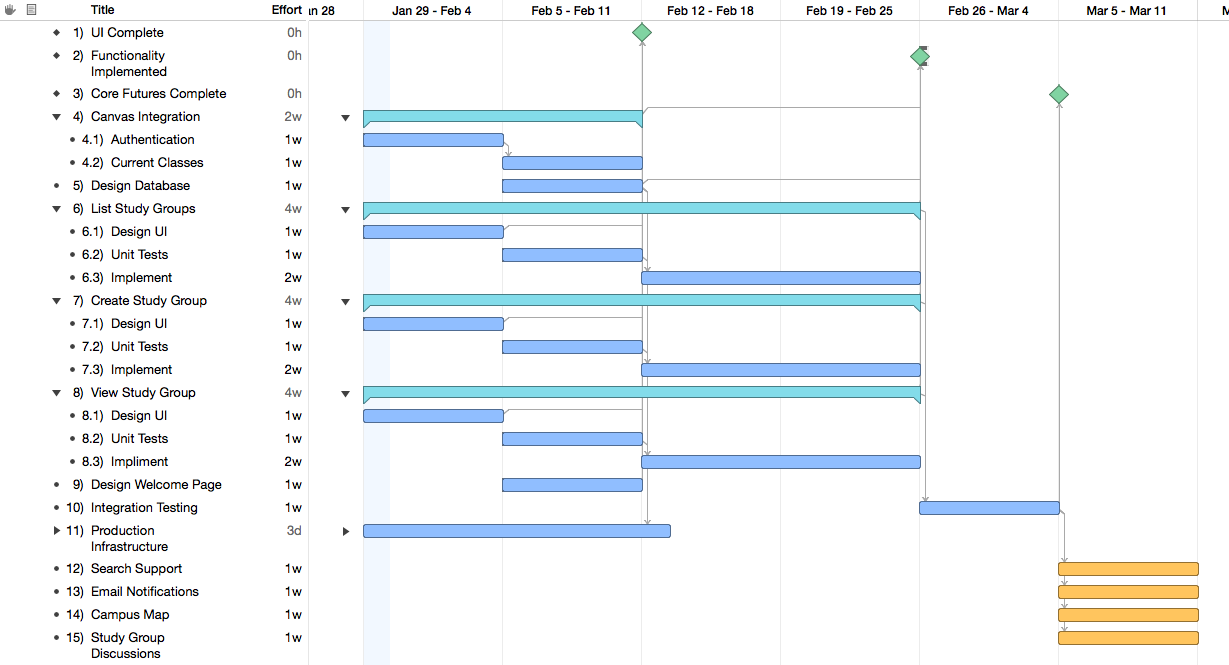
\includegraphics[width=\linewidth]{StudyUp_Gantt.png}
  \caption{Gantt Schedule}
  \label{gantt}
\end{figure}

\subsubsection{Project Tracking}
Project tracking will be done using GitHub issues and milestones. Team members will be assigned tasks (issues) to be completed by a date as specified by milestones. Tasks not completed in time will become the top priority to ensure the project stays on track. More members may be assigned to the task if it is determined to be beneficial. GitHub Insights will also be used to track team member contributions as the project progresses.

\subsubsection{Risk Management}
The are multiple risks that affect the successful and timely implementation of this project. These risks include, time allocation, experience, and communication.

Time allocation for team members to work on the project is the primary risk. In order for this project the be completed on time team members must dedicate an adequate amount of hours per week to complete tasks. At the minimum 8 hours should be allocated to working on this project as is expected with a 4 credit class. More time may be required to complete tasks on schedule.

Another risk that compounds with time allocation is experience. Team members who do not have experience working on large projects or technology being used requires more overhead. This can be mitigated to a degree by providing resources to aid in their learning. Having less experience though does require more time and assistance with the development process.

The final risk is communicating with team members. Working on a project of this size requires constant team communication to work effectively. This risk has largely been mitigated by having phone number and email of team members. As well as uploading work done to GitHub to monitor task progress.

\section{Meeting Report}
Our group met at the library on Friday January 26th. Unfortunately, two of our group members have been unresponsive so we prepared for the worst case, which is having to complete the project with a three person group. Since our meeting on Saturday night, Moyez responded to our initial welcome email and was unresponsive due to sickness. The progress we have made in the first week includes, learning about the skill sets our group members have, deciding what framework we will use, and preparing for the project by getting the proper software.

Our plans and goals for the next week include drawing up mocks of the StudyUp graphical user interface, determining the structure and layout of the main page,learning how to use the Canvas API, coding the basic HTML structure of the application, and delegating tasks. 

Thus far, Yukon and Chandler were the group members who came up with the idea of StudyUp and drafted the initial project proposal. Yukon organized the group meeting and contacted other members. During the meeting, Yukon, Chandler, and Calvin discussed and decided on the basic features and use cases that were discussed in this report. These three members are also the contributing members to the report.

\end{document}
